% Options for packages loaded elsewhere
\PassOptionsToPackage{unicode}{hyperref}
\PassOptionsToPackage{hyphens}{url}
%
\documentclass[
  ignorenonframetext,
]{beamer}
\usepackage{pgfpages}
\setbeamertemplate{caption}[numbered]
\setbeamertemplate{caption label separator}{: }
\setbeamercolor{caption name}{fg=normal text.fg}
\beamertemplatenavigationsymbolsempty
% Prevent slide breaks in the middle of a paragraph
\widowpenalties 1 10000
\raggedbottom
\setbeamertemplate{part page}{
  \centering
  \begin{beamercolorbox}[sep=16pt,center]{part title}
    \usebeamerfont{part title}\insertpart\par
  \end{beamercolorbox}
}
\setbeamertemplate{section page}{
  \centering
  \begin{beamercolorbox}[sep=12pt,center]{part title}
    \usebeamerfont{section title}\insertsection\par
  \end{beamercolorbox}
}
\setbeamertemplate{subsection page}{
  \centering
  \begin{beamercolorbox}[sep=8pt,center]{part title}
    \usebeamerfont{subsection title}\insertsubsection\par
  \end{beamercolorbox}
}
\AtBeginPart{
  \frame{\partpage}
}
\AtBeginSection{
  \ifbibliography
  \else
    \frame{\sectionpage}
  \fi
}
\AtBeginSubsection{
  \frame{\subsectionpage}
}

\usepackage{amsmath,amssymb}
\usepackage{iftex}
\ifPDFTeX
  \usepackage[T1]{fontenc}
  \usepackage[utf8]{inputenc}
  \usepackage{textcomp} % provide euro and other symbols
\else % if luatex or xetex
  \usepackage{unicode-math}
  \defaultfontfeatures{Scale=MatchLowercase}
  \defaultfontfeatures[\rmfamily]{Ligatures=TeX,Scale=1}
\fi
\usepackage{lmodern}
\usetheme[]{Boadilla}
\usecolortheme{rose}
\ifPDFTeX\else  
    % xetex/luatex font selection
\fi
% Use upquote if available, for straight quotes in verbatim environments
\IfFileExists{upquote.sty}{\usepackage{upquote}}{}
\IfFileExists{microtype.sty}{% use microtype if available
  \usepackage[]{microtype}
  \UseMicrotypeSet[protrusion]{basicmath} % disable protrusion for tt fonts
}{}
\makeatletter
\@ifundefined{KOMAClassName}{% if non-KOMA class
  \IfFileExists{parskip.sty}{%
    \usepackage{parskip}
  }{% else
    \setlength{\parindent}{0pt}
    \setlength{\parskip}{6pt plus 2pt minus 1pt}}
}{% if KOMA class
  \KOMAoptions{parskip=half}}
\makeatother
\usepackage{xcolor}
\newif\ifbibliography
\setlength{\emergencystretch}{3em} % prevent overfull lines
\setcounter{secnumdepth}{-\maxdimen} % remove section numbering

\usepackage{color}
\usepackage{fancyvrb}
\newcommand{\VerbBar}{|}
\newcommand{\VERB}{\Verb[commandchars=\\\{\}]}
\DefineVerbatimEnvironment{Highlighting}{Verbatim}{commandchars=\\\{\}}
% Add ',fontsize=\small' for more characters per line
\usepackage{framed}
\definecolor{shadecolor}{RGB}{241,243,245}
\newenvironment{Shaded}{\begin{snugshade}}{\end{snugshade}}
\newcommand{\AlertTok}[1]{\textcolor[rgb]{0.68,0.00,0.00}{#1}}
\newcommand{\AnnotationTok}[1]{\textcolor[rgb]{0.37,0.37,0.37}{#1}}
\newcommand{\AttributeTok}[1]{\textcolor[rgb]{0.40,0.45,0.13}{#1}}
\newcommand{\BaseNTok}[1]{\textcolor[rgb]{0.68,0.00,0.00}{#1}}
\newcommand{\BuiltInTok}[1]{\textcolor[rgb]{0.00,0.23,0.31}{#1}}
\newcommand{\CharTok}[1]{\textcolor[rgb]{0.13,0.47,0.30}{#1}}
\newcommand{\CommentTok}[1]{\textcolor[rgb]{0.37,0.37,0.37}{#1}}
\newcommand{\CommentVarTok}[1]{\textcolor[rgb]{0.37,0.37,0.37}{\textit{#1}}}
\newcommand{\ConstantTok}[1]{\textcolor[rgb]{0.56,0.35,0.01}{#1}}
\newcommand{\ControlFlowTok}[1]{\textcolor[rgb]{0.00,0.23,0.31}{#1}}
\newcommand{\DataTypeTok}[1]{\textcolor[rgb]{0.68,0.00,0.00}{#1}}
\newcommand{\DecValTok}[1]{\textcolor[rgb]{0.68,0.00,0.00}{#1}}
\newcommand{\DocumentationTok}[1]{\textcolor[rgb]{0.37,0.37,0.37}{\textit{#1}}}
\newcommand{\ErrorTok}[1]{\textcolor[rgb]{0.68,0.00,0.00}{#1}}
\newcommand{\ExtensionTok}[1]{\textcolor[rgb]{0.00,0.23,0.31}{#1}}
\newcommand{\FloatTok}[1]{\textcolor[rgb]{0.68,0.00,0.00}{#1}}
\newcommand{\FunctionTok}[1]{\textcolor[rgb]{0.28,0.35,0.67}{#1}}
\newcommand{\ImportTok}[1]{\textcolor[rgb]{0.00,0.46,0.62}{#1}}
\newcommand{\InformationTok}[1]{\textcolor[rgb]{0.37,0.37,0.37}{#1}}
\newcommand{\KeywordTok}[1]{\textcolor[rgb]{0.00,0.23,0.31}{#1}}
\newcommand{\NormalTok}[1]{\textcolor[rgb]{0.00,0.23,0.31}{#1}}
\newcommand{\OperatorTok}[1]{\textcolor[rgb]{0.37,0.37,0.37}{#1}}
\newcommand{\OtherTok}[1]{\textcolor[rgb]{0.00,0.23,0.31}{#1}}
\newcommand{\PreprocessorTok}[1]{\textcolor[rgb]{0.68,0.00,0.00}{#1}}
\newcommand{\RegionMarkerTok}[1]{\textcolor[rgb]{0.00,0.23,0.31}{#1}}
\newcommand{\SpecialCharTok}[1]{\textcolor[rgb]{0.37,0.37,0.37}{#1}}
\newcommand{\SpecialStringTok}[1]{\textcolor[rgb]{0.13,0.47,0.30}{#1}}
\newcommand{\StringTok}[1]{\textcolor[rgb]{0.13,0.47,0.30}{#1}}
\newcommand{\VariableTok}[1]{\textcolor[rgb]{0.07,0.07,0.07}{#1}}
\newcommand{\VerbatimStringTok}[1]{\textcolor[rgb]{0.13,0.47,0.30}{#1}}
\newcommand{\WarningTok}[1]{\textcolor[rgb]{0.37,0.37,0.37}{\textit{#1}}}

\providecommand{\tightlist}{%
  \setlength{\itemsep}{0pt}\setlength{\parskip}{0pt}}\usepackage{longtable,booktabs,array}
\usepackage{calc} % for calculating minipage widths
\usepackage{caption}
% Make caption package work with longtable
\makeatletter
\def\fnum@table{\tablename~\thetable}
\makeatother
\usepackage{graphicx}
\makeatletter
\def\maxwidth{\ifdim\Gin@nat@width>\linewidth\linewidth\else\Gin@nat@width\fi}
\def\maxheight{\ifdim\Gin@nat@height>\textheight\textheight\else\Gin@nat@height\fi}
\makeatother
% Scale images if necessary, so that they will not overflow the page
% margins by default, and it is still possible to overwrite the defaults
% using explicit options in \includegraphics[width, height, ...]{}
\setkeys{Gin}{width=\maxwidth,height=\maxheight,keepaspectratio}
% Set default figure placement to htbp
\makeatletter
\def\fps@figure{htbp}
\makeatother

\makeatletter
\makeatother
\makeatletter
\makeatother
\makeatletter
\@ifpackageloaded{caption}{}{\usepackage{caption}}
\AtBeginDocument{%
\ifdefined\contentsname
  \renewcommand*\contentsname{Table of contents}
\else
  \newcommand\contentsname{Table of contents}
\fi
\ifdefined\listfigurename
  \renewcommand*\listfigurename{List of Figures}
\else
  \newcommand\listfigurename{List of Figures}
\fi
\ifdefined\listtablename
  \renewcommand*\listtablename{List of Tables}
\else
  \newcommand\listtablename{List of Tables}
\fi
\ifdefined\figurename
  \renewcommand*\figurename{Figure}
\else
  \newcommand\figurename{Figure}
\fi
\ifdefined\tablename
  \renewcommand*\tablename{Table}
\else
  \newcommand\tablename{Table}
\fi
}
\@ifpackageloaded{float}{}{\usepackage{float}}
\floatstyle{ruled}
\@ifundefined{c@chapter}{\newfloat{codelisting}{h}{lop}}{\newfloat{codelisting}{h}{lop}[chapter]}
\floatname{codelisting}{Listing}
\newcommand*\listoflistings{\listof{codelisting}{List of Listings}}
\makeatother
\makeatletter
\@ifpackageloaded{caption}{}{\usepackage{caption}}
\@ifpackageloaded{subcaption}{}{\usepackage{subcaption}}
\makeatother
\makeatletter
\@ifpackageloaded{tcolorbox}{}{\usepackage[skins,breakable]{tcolorbox}}
\makeatother
\makeatletter
\@ifundefined{shadecolor}{\definecolor{shadecolor}{rgb}{.97, .97, .97}}
\makeatother
\makeatletter
\makeatother
\makeatletter
\makeatother
\ifLuaTeX
  \usepackage{selnolig}  % disable illegal ligatures
\fi
\IfFileExists{bookmark.sty}{\usepackage{bookmark}}{\usepackage{hyperref}}
\IfFileExists{xurl.sty}{\usepackage{xurl}}{} % add URL line breaks if available
\urlstyle{same} % disable monospaced font for URLs
\hypersetup{
  pdftitle={Motivation and Big-O},
  pdfauthor={Salaar Liaqat},
  hidelinks,
  pdfcreator={LaTeX via pandoc}}

\title{Motivation and Big-O}
\author{Salaar Liaqat}
\date{}
\institute{Data Sciences Institute, UofT}

\begin{document}
\frame{\titlepage}
\ifdefined\Shaded\renewenvironment{Shaded}{\begin{tcolorbox}[boxrule=0pt, enhanced, frame hidden, borderline west={3pt}{0pt}{shadecolor}, interior hidden, sharp corners, breakable]}{\end{tcolorbox}}\fi

\begin{frame}{Outline}
\protect\hypertarget{outline}{}
\begin{itemize}
\item
  Motivation
\item
  Time Complexity: Introduction to Big-O Notation
\item
  Average, Best, and Worst Case
\item
  Space Complexity
\end{itemize}
\end{frame}

\begin{frame}{About Me}
\protect\hypertarget{about-me}{}
\begin{itemize}
\item
  PhD candidate in the Department of Computer Science at UofT
\item
  Thesis is on remote patient monitoring using wearables and mobile
  devices
\item
  Did BSc from Vancouver (SFU) and MSc from UofT
\item
  Co-Founder of a remote patient monitoring startup (Tabiat)
\end{itemize}
\end{frame}

\begin{frame}{Why should a Data Scientist take this Course?}
\protect\hypertarget{why-should-a-data-scientist-take-this-course}{}
\begin{itemize}
\item
  Problem solving. This course provides you with a framework to solve
  coding problems you may encounter in your career.
\item
  Efficient programs. We want to write programs that scale well with big
  data.
\item
  Interview preparation. Many data science jobs require a technical
  interview, which involes solving algorithms problems.
\end{itemize}
\end{frame}

\begin{frame}{Learning Objectives}
\protect\hypertarget{learning-objectives}{}
\begin{itemize}
\item
  Assess options and choices around methods to solve problems and data
  representation methods using Big-O notation.
\item
  Develop comfort with recursive functions.
\item
  Decide on appropriate methods to represent data for a problem.
\item
  Take a client-led problem and translate it into an optimization
  problem.
\item
  Identify why code is running slowly and know how to improve its
  performance.
\end{itemize}
\end{frame}

\hypertarget{motivating-code-demos}{%
\section{Motivating Code Demos}\label{motivating-code-demos}}

\begin{frame}[fragile]{What are Algorithms and Data Structures}
\protect\hypertarget{what-are-algorithms-and-data-structures}{}
\begin{itemize}
\item
  An \textbf{algorithm} is a procedure to solve a problem

  \begin{itemize}
  \item
    Sort a data observations from smallest to largest
  \item
    Find the nearest neighbor to a data point
  \item
    How fast is each algorithm?
  \end{itemize}
\item
  A \textbf{data structure} is a concrete method to store some data.

  \begin{itemize}
  \item
    A pandas data set is a good way to store observations with many
    features.
  \item
    How much space does the data sturcture need? How long does it take
    to access each observation?
  \end{itemize}
\end{itemize}

\begin{Shaded}
\begin{Highlighting}[]
\ImportTok{import}\NormalTok{ numpy }\ImportTok{as}\NormalTok{ np}
\ImportTok{import}\NormalTok{ timeit}
\ImportTok{import}\NormalTok{ random}
\end{Highlighting}
\end{Shaded}
\end{frame}

\begin{frame}[fragile]{Loop Versus Vectorized Operations}
\protect\hypertarget{loop-versus-vectorized-operations}{}
\begin{Shaded}
\begin{Highlighting}[]
\NormalTok{size }\OperatorTok{=} \DecValTok{10}\OperatorTok{**}\DecValTok{4}

\CommentTok{\# Using Python lists}
\NormalTok{list\_a }\OperatorTok{=} \BuiltInTok{list}\NormalTok{(}\BuiltInTok{range}\NormalTok{(size))}
\NormalTok{list\_b }\OperatorTok{=} \BuiltInTok{list}\NormalTok{(}\BuiltInTok{range}\NormalTok{(size))}

\CommentTok{\# Using NumPy arrays}
\NormalTok{array\_a }\OperatorTok{=}\NormalTok{ np.arange(size)}
\NormalTok{array\_b }\OperatorTok{=}\NormalTok{ np.arange(size)}

\CommentTok{\# Timing for list addition}
\NormalTok{list\_time }\OperatorTok{=}\NormalTok{ timeit.timeit(}\KeywordTok{lambda}\NormalTok{: }
\NormalTok{  [a }\OperatorTok{+}\NormalTok{ b }\ControlFlowTok{for}\NormalTok{ a, b }\KeywordTok{in} \BuiltInTok{zip}\NormalTok{(list\_a, list\_b)], number}\OperatorTok{=}\DecValTok{1}\NormalTok{)}

\CommentTok{\# Timing for vectorized array addition}
\NormalTok{array\_time }\OperatorTok{=}\NormalTok{ timeit.timeit(}\KeywordTok{lambda}\NormalTok{: }
\NormalTok{  array\_a }\OperatorTok{+}\NormalTok{ array\_b, number }\OperatorTok{=} \DecValTok{1}\NormalTok{)}
\end{Highlighting}
\end{Shaded}
\end{frame}

\begin{frame}[fragile]{Loop Versus Vectorized Operations}
\protect\hypertarget{loop-versus-vectorized-operations-1}{}
We will learn about what vectorized is in lecture 6.

\begin{Shaded}
\begin{Highlighting}[]
\BuiltInTok{print}\NormalTok{(}\SpecialStringTok{f"List Addition: }\SpecialCharTok{\{}\NormalTok{list\_time}\SpecialCharTok{:.6f\}}\SpecialStringTok{ seconds"}\NormalTok{)}
\BuiltInTok{print}\NormalTok{(}\SpecialStringTok{f"Vectorized Addition: }\SpecialCharTok{\{}\NormalTok{array\_time}\SpecialCharTok{:.6f\}}\SpecialStringTok{ seconds"}\NormalTok{)}
\end{Highlighting}
\end{Shaded}

\begin{verbatim}
List Addition: 0.000337 seconds
Vectorized Addition: 0.000052 seconds
\end{verbatim}

\begin{itemize}
\item
  Why was the NumPy vectorized operation much faster?
\item
  How can we describe how much faster the vectorized operation is?
\item
  This is useful in many iterative algorithms, such as gradient descent.
\end{itemize}
\end{frame}

\begin{frame}[fragile]{Search in List Versus Set}
\protect\hypertarget{search-in-list-versus-set}{}
We will learn about searching and sorting in lecture 2.

\begin{Shaded}
\begin{Highlighting}[]
\CommentTok{\# Python list}
\NormalTok{list\_time }\OperatorTok{=}\NormalTok{ timeit.timeit(}\KeywordTok{lambda}\NormalTok{:}
  \OperatorTok{{-}}\DecValTok{1} \KeywordTok{in}\NormalTok{ list\_a, number }\OperatorTok{=} \DecValTok{1}\NormalTok{)}
  
\CommentTok{\# Python set}
\NormalTok{set\_a }\OperatorTok{=} \BuiltInTok{set}\NormalTok{(}\BuiltInTok{range}\NormalTok{(size))}
\NormalTok{set\_time }\OperatorTok{=}\NormalTok{ timeit.timeit(}\KeywordTok{lambda}\NormalTok{:}
  \OperatorTok{{-}}\DecValTok{1} \KeywordTok{in}\NormalTok{ set\_a, number }\OperatorTok{=} \DecValTok{1}\NormalTok{)}
\end{Highlighting}
\end{Shaded}
\end{frame}

\begin{frame}[fragile]{Search in List Versus Set}
\protect\hypertarget{search-in-list-versus-set-1}{}
\begin{Shaded}
\begin{Highlighting}[]
\BuiltInTok{print}\NormalTok{(}\SpecialStringTok{f"List Search: }\SpecialCharTok{\{}\NormalTok{list\_time}\SpecialCharTok{:.6f\}}\SpecialStringTok{ seconds"}\NormalTok{)}
\BuiltInTok{print}\NormalTok{(}\SpecialStringTok{f"Set Search: }\SpecialCharTok{\{}\NormalTok{set\_time}\SpecialCharTok{:.6f\}}\SpecialStringTok{ seconds"}\NormalTok{)}
\end{Highlighting}
\end{Shaded}

\begin{verbatim}
List Search: 0.000036 seconds
Set Search: 0.000000 seconds
\end{verbatim}

\begin{itemize}
\item
  Why was the set search much faster?
\item
  How can we describe how much faster the vectorized operation is?
\item
  What are the pros and cons of choosing each data structure?
\end{itemize}
\end{frame}

\begin{frame}[fragile]{Selection Sort Versus Python Sort}
\protect\hypertarget{selection-sort-versus-python-sort}{}
For context, selection sort is a naive sorting algorithm, while Python
implements Tim Sort for the default search function.

\begin{Shaded}
\begin{Highlighting}[]
\KeywordTok{def}\NormalTok{ selection\_sort(arr):}
\NormalTok{  n }\OperatorTok{=} \BuiltInTok{len}\NormalTok{(arr)}
  
  \ControlFlowTok{for}\NormalTok{ i }\KeywordTok{in} \BuiltInTok{range}\NormalTok{(n):}
\NormalTok{    min\_index }\OperatorTok{=}\NormalTok{ i}
    \ControlFlowTok{for}\NormalTok{ j }\KeywordTok{in} \BuiltInTok{range}\NormalTok{(i}\OperatorTok{+}\DecValTok{1}\NormalTok{, n):}
      \ControlFlowTok{if}\NormalTok{ arr[j] }\OperatorTok{\textless{}}\NormalTok{ arr[min\_index]:}
\NormalTok{        min\_index }\OperatorTok{=}\NormalTok{ j}
        
\NormalTok{    arr[i], arr[min\_index] }\OperatorTok{=}\NormalTok{ arr[min\_index], arr[i]}
\end{Highlighting}
\end{Shaded}
\end{frame}

\begin{frame}[fragile]{Selection Sort Versus Python Sort}
\protect\hypertarget{selection-sort-versus-python-sort-1}{}
\begin{Shaded}
\begin{Highlighting}[]
\NormalTok{random.shuffle(list\_a)}
\NormalTok{rand\_list }\OperatorTok{=}\NormalTok{ list\_a.copy()}

\NormalTok{sel\_time }\OperatorTok{=}\NormalTok{ timeit.timeit(}\KeywordTok{lambda}\NormalTok{:}
\NormalTok{  selection\_sort(rand\_list.copy()), number }\OperatorTok{=} \DecValTok{1}\NormalTok{)}
  
\NormalTok{py\_time }\OperatorTok{=}\NormalTok{ timeit.timeit(}\KeywordTok{lambda}\NormalTok{:}
  \BuiltInTok{sorted}\NormalTok{(rand\_list.copy()), number }\OperatorTok{=} \DecValTok{1}\NormalTok{)}
\end{Highlighting}
\end{Shaded}
\end{frame}

\begin{frame}[fragile]{Selection Sort Versus Python Sort}
\protect\hypertarget{selection-sort-versus-python-sort-2}{}
\begin{Shaded}
\begin{Highlighting}[]
\BuiltInTok{print}\NormalTok{(}\SpecialStringTok{f"Selection sort: }\SpecialCharTok{\{}\NormalTok{sel\_time}\SpecialCharTok{:.6f\}}\SpecialStringTok{ seconds"}\NormalTok{)}
\BuiltInTok{print}\NormalTok{(}\SpecialStringTok{f"Tim sort: }\SpecialCharTok{\{}\NormalTok{py\_time}\SpecialCharTok{:.6f\}}\SpecialStringTok{ seconds"}\NormalTok{)}
\end{Highlighting}
\end{Shaded}

\begin{verbatim}
Selection sort: 1.625933 seconds
Tim sort: 0.000862 seconds
\end{verbatim}

\begin{itemize}
\item
  Why was selection sort much slower than Tim sort (not in detail)?
\item
  If we double the size of the list, how much slower will the code be in
  each case?
\end{itemize}
\end{frame}

\hypertarget{time-complexity-introduction-to-big-o-notation}{%
\section{Time Complexity: Introduction to Big-O
Notation}\label{time-complexity-introduction-to-big-o-notation}}

\begin{frame}{An example}
\protect\hypertarget{an-example}{}
\begin{itemize}
\item
  Imagine you are writing an algorithm to search for a landing position
  for a rocket. You want it to be simple (to avoid bugs) and fast (since
  you only have 10 seconds to find a site). \footnote<.->{Example from
    Grokking Algorithms}
\item
  It takes 1 millisecond to check each element. You decide to test a
  simple search and binary search on 100 elements (more on these methods
  later).

  \begin{itemize}
  \tightlist
  \item
    Simple search takes 100ms. Binary search takes 7ms.
  \end{itemize}
\item
  Then you test binary search with 1 billion elements and it takes 32ms.

  \begin{itemize}
  \tightlist
  \item
    Binary search is about 15 times faster than simple search, because
    simple search took 100 ms with 100 elements, and binary search took
    7 ms. So simple search will take 30 × 15 = 450ms with 1 billion
    elements.
  \end{itemize}
\item
  Since that is within your threshold, you decide to go with simple
  search. \textbf{Is this correct?}
\end{itemize}
\end{frame}

\begin{frame}{A practical example}
\protect\hypertarget{a-practical-example}{}
\begin{itemize}
\tightlist
\item
  Definitely wrong!!
\item
  The run time of different algorithms can grow at different rates.
\item
  Big-O tells us how run time increases as the list size increases.
\end{itemize}

\begin{block}{Comparing run times of simple and binary search}
\protect\hypertarget{comparing-run-times-of-simple-and-binary-search}{}
\begin{longtable}[]{@{}lll@{}}
\toprule\noalign{}
Elements & Simple Search & Binary Search \\
\midrule\noalign{}
\endhead
100 & 100 ms & 7 ms \\
10,000 & 10 s & 14 ms \\
1,000,000,000 & 11 days & 32 ms \\
\bottomrule\noalign{}
\end{longtable}
\end{block}
\end{frame}

\begin{frame}{Big-O Notation}
\protect\hypertarget{big-o-notation}{}
\begin{itemize}
\item
  Big-O tells you how fast an algorithm is in terms of the number of
  operations, \(n\).
\item
  Simple search needs to take each element, so it will take \(n\)
  operations. The run time in Big-O notation is \(O(n)\).
\item
  Binary search needs log \(n\) operations, so the run time in Big-O
  notation is \(O(\text{log}n)\)

  \begin{itemize}
  \tightlist
  \item
    Note: log in computer science usually refers to log base 2.
  \end{itemize}
\end{itemize}
\end{frame}

\begin{frame}{Big-O is Upper Bound Run Time}
\protect\hypertarget{big-o-is-upper-bound-run-time}{}
\begin{itemize}
\item
  Big-O notation is about the \emph{worst-case} scenario.

  \begin{itemize}
  \tightlist
  \item
    If you were conducting linear search through a phone book, even if
    you were looking for Abe Aberdeen, it is still considered \(O(n)\).
  \end{itemize}
\item
  Formally, it characterizes an upper bound on the asymptotic behavior
  of the run time.
\item
  For example, the function \(7n^3 + 30n^2 - 200n + 9\) has
  highest-order term \(7n^3\). The function's growth rate is \(n^3\)
  because the function grows no faster than \(n^3\). The Big-O is
  \(O(n^3)\).
\end{itemize}
\end{frame}

\begin{frame}{Common Big-O Run Times}
\protect\hypertarget{common-big-o-run-times}{}
Here are seven Big-O run times that you'll encounter frequently, sorted
from fasted to slowest.

\begin{columns}[T]
\begin{column}{0.4\textwidth}
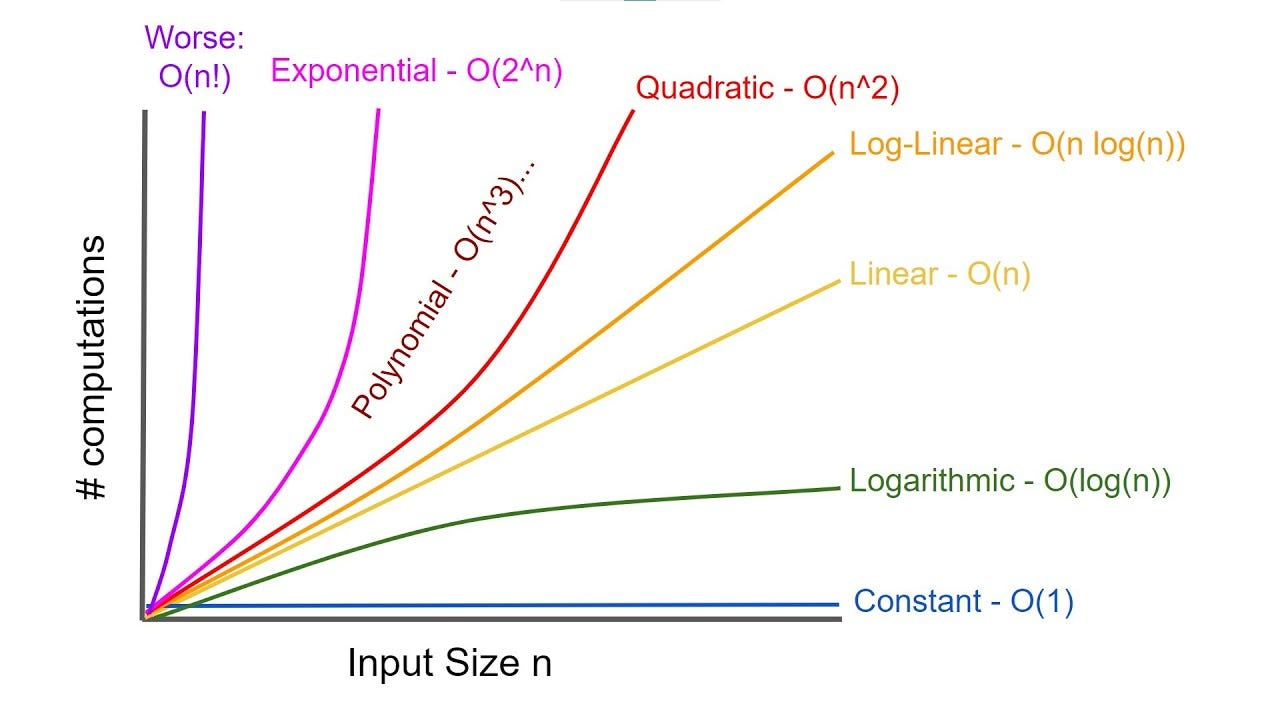
\includegraphics{images/big-o-viz.jpg}
\end{column}

\begin{column}{0.6\textwidth}
\begin{itemize}
\item
  \(O(1)\), known as \emph{constant time}. Ex: addition, division
\item
  \(O(\text{log}n)\), known as \emph{logarithmic time}. Ex: binary
  search
\item
  \(O(n)\), known as \emph{linear time}. Ex: Linear search
\item
  \(O(n\text{log}n)\). Ex: Tim Sort
\item
  \(O(n^2)\), known as \emph{quadratic time}. Ex: Selection sort.
\item
  \(O(2^n)\), known as \emph{exponential time}. Ex: Naive recursive
  solution for nth Fibonacci number
\item
  \(O(n!)\), known as \emph{factorial time}. Ex. Traveling salesperson
\end{itemize}
\end{column}
\end{columns}
\end{frame}

\begin{frame}[fragile]{Determining Time Complexity}
\protect\hypertarget{determining-time-complexity}{}
Consider the following code. How can you determine the Big-O?

\begin{Shaded}
\begin{Highlighting}[]
\KeywordTok{def}\NormalTok{ f(n):}
  \ControlFlowTok{for}\NormalTok{ i }\KeywordTok{in} \BuiltInTok{range}\NormalTok{(n):}
    \ControlFlowTok{for}\NormalTok{ j }\KeywordTok{in} \BuiltInTok{range}\NormalTok{(n):}
      \BuiltInTok{print}\NormalTok{(i, j)}
\end{Highlighting}
\end{Shaded}
\end{frame}

\begin{frame}[fragile]{Determining Time Complexity}
\protect\hypertarget{determining-time-complexity-1}{}
\begin{itemize}
\item
  With ``raw'' Python code, you can usually count the number of nested
  \texttt{for} loops to determine the Big-O

  \begin{itemize}
  \item
    A loop gives \(O(n)\)
  \item
    A nested loop gives \(O(n^2)\)
  \end{itemize}
\item
  It's usually not so simple in Data Science because of packages we use.
\item
  There are many factors affecting the constants in your run time

  \begin{itemize}
  \item
    How complicated is each step? Is it \(n\) or \(2000n\)?
  \item
    How are your algorithms implemented? Is your programming language
    fast? Are your libraries fast?
  \end{itemize}
\item
  Implementation issues will be covered later in the course.
\end{itemize}
\end{frame}

\begin{frame}[fragile]{Big-O with Two Variables}
\protect\hypertarget{big-o-with-two-variables}{}
Consider the following code. What is it's Big-O?

\begin{Shaded}
\begin{Highlighting}[]
\KeywordTok{def}\NormalTok{ fun(n,m):}
  \ControlFlowTok{for}\NormalTok{ i }\KeywordTok{in} \BuiltInTok{range}\NormalTok{(n):}
    \ControlFlowTok{for}\NormalTok{ j }\KeywordTok{in} \BuiltInTok{range}\NormalTok{(m):}
      \BuiltInTok{print}\NormalTok{(}\StringTok{"Hello"}\NormalTok{)}
\end{Highlighting}
\end{Shaded}
\end{frame}

\begin{frame}{Big-O with Two Variables}
\protect\hypertarget{big-o-with-two-variables-1}{}
\begin{itemize}
\item
  The time complexity here is \(O(nm)\).

  \begin{itemize}
  \tightlist
  \item
    If \(n = m\), then \(O(n^2)\).
  \end{itemize}
\item
  All terms should be combined into one Big-O

  \begin{itemize}
  \item
    \(O(nm)\) is correct and \(O(n)O(m)\) is incorrect.
  \item
    \(O(n + m)\) is correct and \(O(n) + O(m)\) is incorrect.
  \item
    \(O(n^2 + mn + m)\) is written as \(O(n^2 + nm)\). We can't throw
    away either term because we don't know which term will dominate.
  \end{itemize}
\item
  Important to think about this when working with datasets.

  \begin{itemize}
  \item
    They have \(n\) rows and \(p\) columns.
  \item
    Can you reason how long it will take to fit a decision tree?
  \end{itemize}
\end{itemize}
\end{frame}

\hypertarget{best-average-and-worst-case}{%
\section{Best, Average, and Worst
Case}\label{best-average-and-worst-case}}

\begin{frame}{Best, Average, and Worst Case}
\protect\hypertarget{best-average-and-worst-case-1}{}
\begin{itemize}
\item
  Big-O deals with worst case.
\item
  If we can develop a notion of an ``average input,'' then we can devise
  the average case of an algorithm.
\item
  Best case is useful to think about the constants in your algorithm.

  \begin{itemize}
  \tightlist
  \item
    \(O(\text{log}n)\) is always faster than \(O(n)\) expect with very
    small \(n\).
  \end{itemize}
\end{itemize}
\end{frame}

\hypertarget{space-complexity}{%
\section{Space Complexity}\label{space-complexity}}

\begin{frame}{What is Space Complexity}
\protect\hypertarget{what-is-space-complexity}{}
\begin{itemize}
\item
  Aside from our algorithm taking too long to run, its also an issue if
  you run out of memory.

  \begin{itemize}
  \item
    Note, memory (RAM), is not the same as disk space.
  \item
    The computer will load data into memory from the disk
  \end{itemize}
\item
  It will be problematic if you need to load 2 billion observations all
  at once.
\item
  We can also analyze space complexity with Big-O notation
\item
  Notice that time complexity is usually about the \emph{algorithm},
  while space complexity is about the \emph{data structure}.
\end{itemize}
\end{frame}

\begin{frame}[fragile]{Examples}
\protect\hypertarget{examples}{}
\begin{itemize}
\item
  Code that prints \texttt{hello\ \{your\ name\}} will have \(O(1)\)
  space.
\item
  Code that sums a list of size \(n\) has \(O(n)\) space.
\item
  You have users on Instagram, and you want to store who follows who.
  The answer depends (why?). The worst case space is \(O(n^2)\)
\end{itemize}
\end{frame}

\hypertarget{recommended-problems-and-references}{%
\section{Recommended Problems and
References}\label{recommended-problems-and-references}}

\begin{frame}{Recommended Problems}
\protect\hypertarget{recommended-problems}{}
\begin{itemize}
\item
  Cormen: Chapter 1 exercises

  \begin{itemize}
  \tightlist
  \item
    1.2-1, 1.2-2, 1.2-3
  \end{itemize}
\item
  Bhargava: Chapter 1 exercises

  \begin{itemize}
  \tightlist
  \item
    1.3 to 1.5
  \end{itemize}
\item
  Additional (for the mathematically inclined)

  \begin{itemize}
  \item
    In CS, log is usually base 2, but a strong distinction is not made
    because \emph{logs of different bases only differ by a constant
    factor} and constants are dropped in Big-O. Show this is true
  \item
    Show that exponents of different bases \textbf{do not} differ by a
    constant factor
  \end{itemize}
\end{itemize}
\end{frame}

\begin{frame}{References}
\protect\hypertarget{references}{}
\begin{itemize}
\item
  Bhargava, A. Y. (2016). \emph{Grokking algorithms: An illustrated
  guide for programmers and other curious people.} Manning. Chapter 1.
\item
  Cormen, T. H. (Ed.). (2009). \emph{Introduction to algorithms} (3rd
  ed). MIT Press. Chapter 1 and 3.
\end{itemize}
\end{frame}



\end{document}
